\section{ニコ書を支えるパーカー}

多くのWeb系企業では、サービスのロゴが入ったグッズを作り配布したりしています。
ニコ書チームもオリジナルのパーカーを制作しました。

\subsection{目的の違い}

一般的に企業がグッズを作るときは、宣伝を目的として、大量に作り無料配布しますが、
ニコ書チームの場合は完全に受注生産で、メンバーが着るために作られました。
もちろん実費負担です。

同じ物を着てチームの一体感を出し結束を固めるのが目的です。
常に着ていられるもの(頻繁に洗わなくて済むもの)である必要があったので、Tシャツは却下されました。
さらに、外に着て行けてロゴがきちんと見えるもの、という条件からパーカーになりました。

\subsection{デザイン}

\begin{figure}[H]
\centering
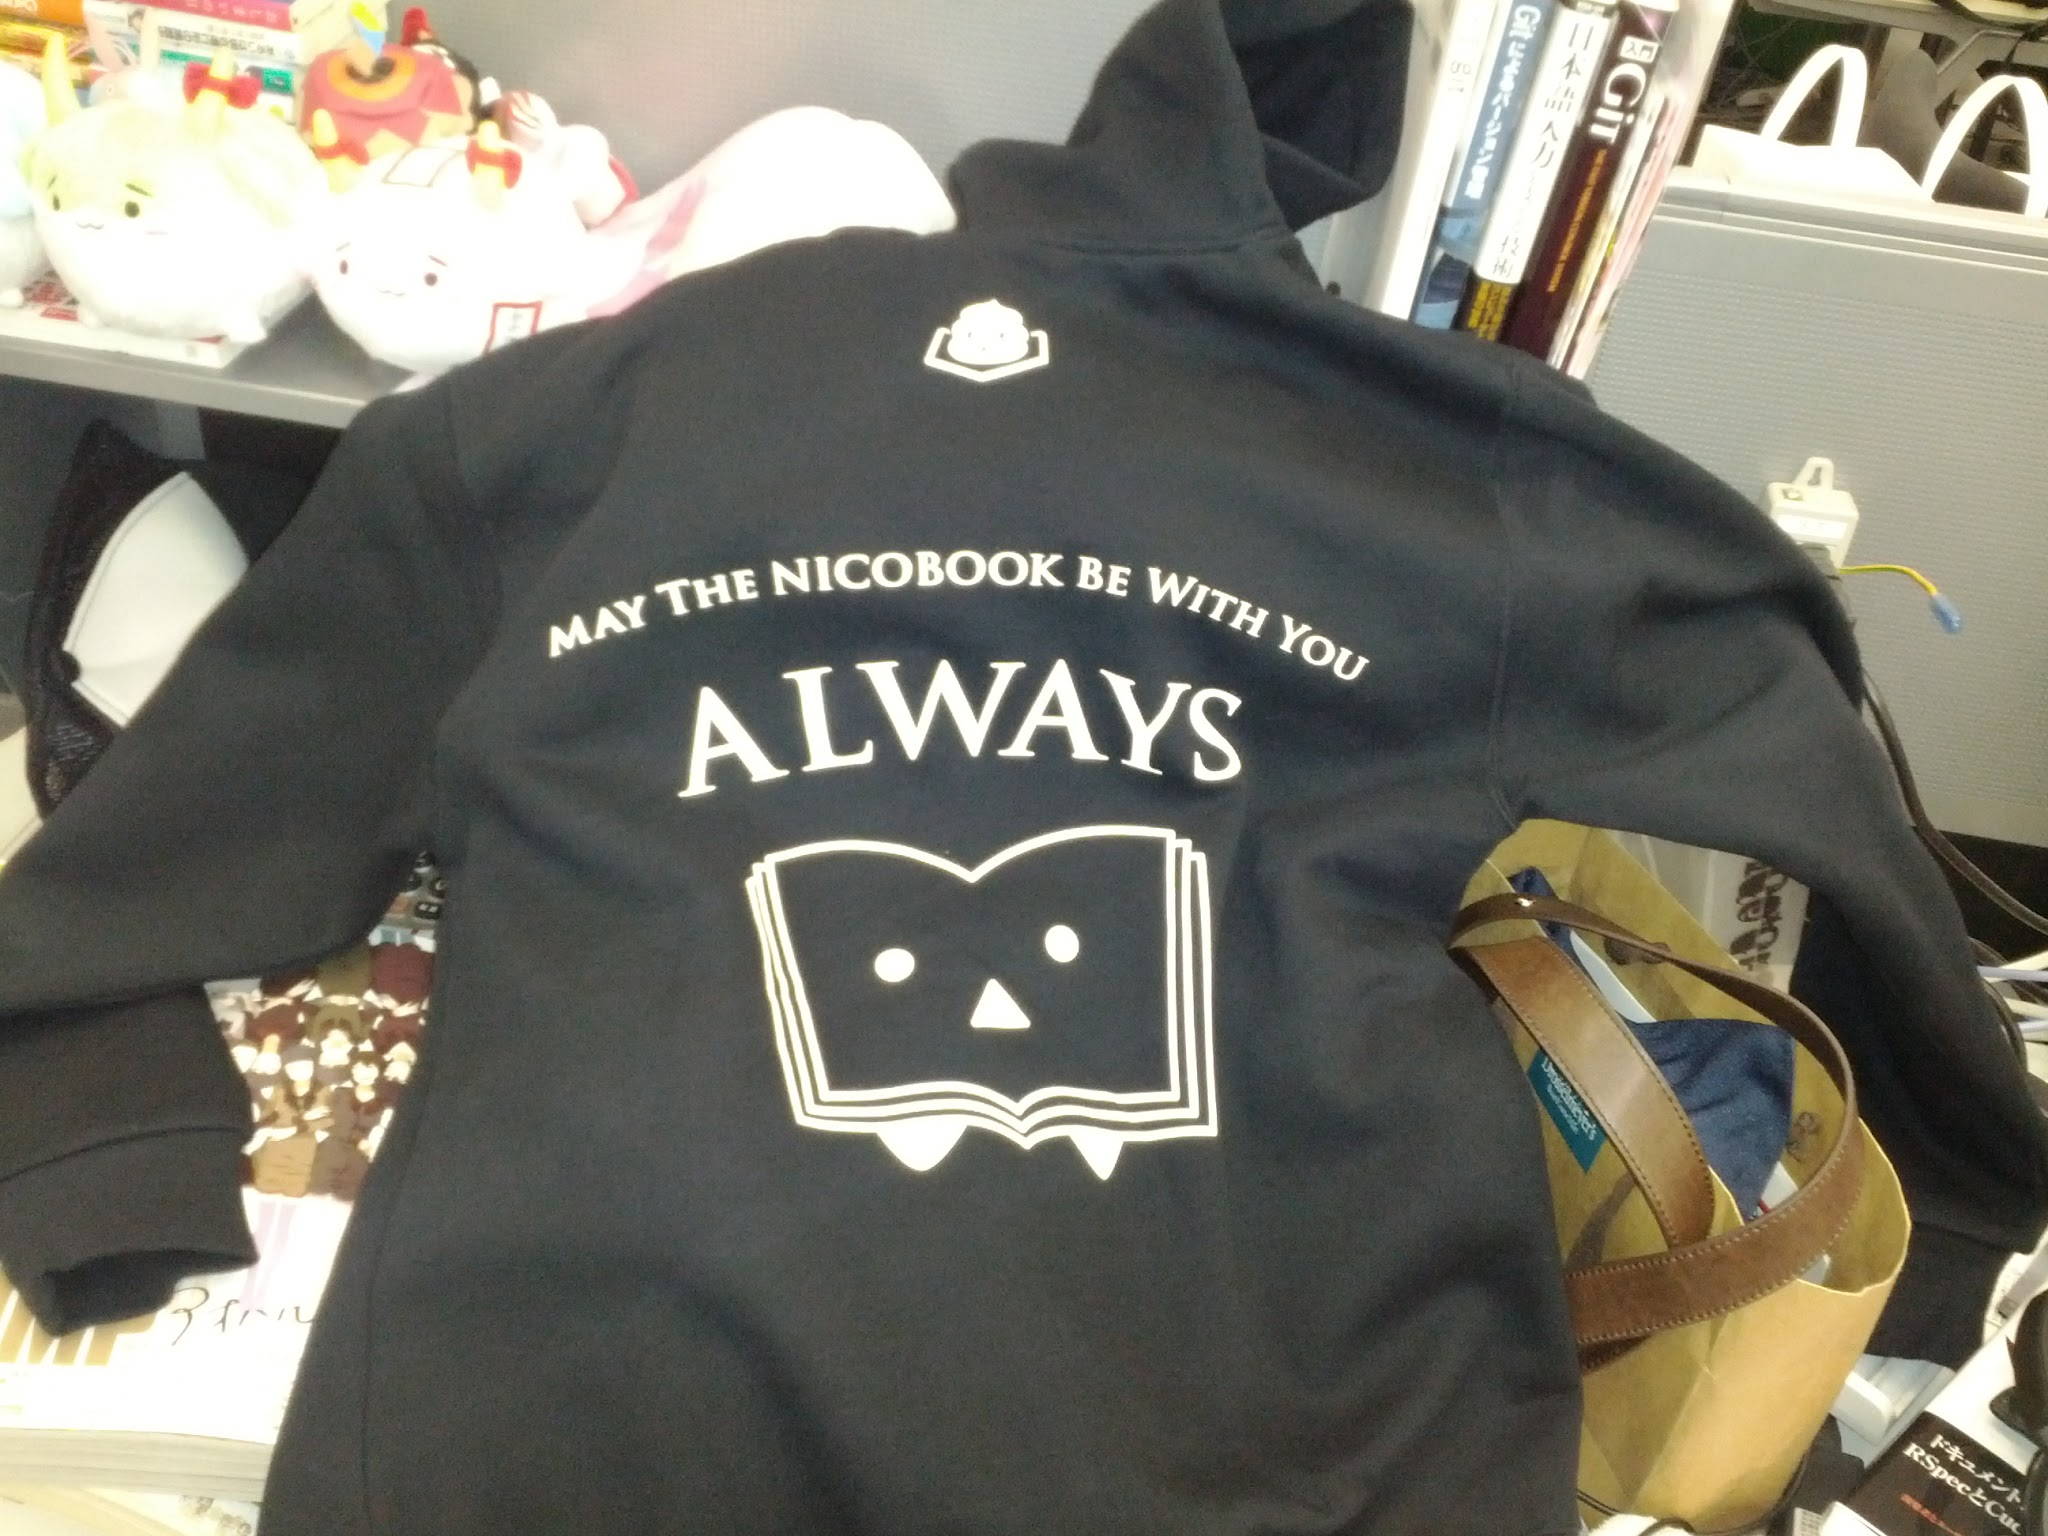
\includegraphics[width=\textwidth]{../images/unko.jpg}
\caption{初代ニコ書パーカー}
\end{figure}

MAY THE NICOBOOK BE WITH YOU ALWAYS
はもちろんスターウォーズのパクリです。
「ニコ書と共にあれ!」という感じです。 その下には公式非公式ロゴ。

フードを被った時だけ顕になる部分には、最初に作られたロゴである「本にうんこ」が隠れています。

\subsection{効果}

1作目のパーカーは非常に肌触りもよく、空気の通りも絶妙で、
寒さの厳しい真冬以外の全シーズンを通して着ることができました。

真夏でも、エアコンで寒い社内はもちろん、朝夕の涼しい時間帯は外でも問題なく着れました。
真夏の昼間でも、近所のコンビニくらいなら平気です。

一年を通してメンバー全員が社内でほぼずっとこのパーカーを着て生活していた結果、
チームのキャラクターも相まって、一部の人にはこのパーカーが恐怖の対象になっているようでした。
北斗の拳で言うところのトゲと肩パットが入ったプロテクターを着てる人に見えるんでしょうか。
正直なところ彼らは汚物なので消毒したかったです。

パーカーは、チーム文化が一番見えやすい形で具現化したものなので、
他のチームから強く憧れられていた一面もあります。
ニコ書チームは非常に成功しているチームで、多くの同僚に憧れを持たれているという実感もあり、
そのチームのロゴを背負い仕事をするということで、
良い緊張感が持続し、質の高い仕事に妥協しないという意識を保てたと思います。
